\documentclass[12pt]{article}
\usepackage[margin=1in]{geometry}
\usepackage{amsmath,amsthm,amssymb,amsfonts}
\usepackage{float}
\usepackage{color}
\usepackage{xcolor}
\usepackage{graphicx}
\usepackage[utf8]{inputenc}
\usepackage{biblatex}
\usepackage{tikz}
\usepackage[page]{appendix}
\usepackage{listings}
\usepackage{mathrsfs}

% tikz style stuff
\usetikzlibrary{arrows}
\tikzstyle{block} = [rectangle, draw, fill=orangeCoral, text width = 1.5em, text centered, minimum height = 2em]
\tikzstyle{blockTurf} = [rectangle, draw, fill=turfGreen!50, text width = 1.5em, text centered, minimum height = 2em]
\tikzstyle{blockAlgae} = [rectangle, draw, fill=algaeRed!45, text width = 1.5em, text centered, minimum height = 2em]
\tikzstyle{blockParrot} = [rectangle, draw, fill=parrotBlue!50, text width = 1.5em, text centered, minimum height = 2em]
\tikzstyle{line} = [thick, ->, >= stealth]
\tikzstyle{dline} = [thick, dashed, ->, >= stealth]
\tikzstyle{noblock} = [rectangle, draw = none]

\definecolor{orangeCoral}{HTML}{FFC996}
\definecolor{turfGreen}{HTML}{BDD2B6}
\definecolor{algaeRed}{HTML}{CF0000}
\definecolor{parrotBlue}{HTML}{A7D0CD}
%----------------------------------------------------

% Code display stuff for lstlisting
\definecolor{codegreen}{rgb}{0,0.6,0}
\definecolor{codegray}{rgb}{0.5,0.5,0.5}
\definecolor{codepurple}{rgb}{0.58,0,0.82}
\definecolor{backcolour}{rgb}{0.95,0.95,0.92}

\lstdefinestyle{mystyle}{
    backgroundcolor=\color{white},   
    commentstyle=\color{codegreen},
    keywordstyle=\color{magenta},
    numberstyle=\tiny\color{codegray},
    stringstyle=\color{codepurple},
    basicstyle=\ttfamily\footnotesize,
    breakatwhitespace=false,         
    breaklines=true,                 
    captionpos=b,                    
    keepspaces=true,                 
    numbers=left,                    
    numbersep=5pt,                  
    showspaces=false,                
    showstringspaces=false,
    showtabs=false,                  
    tabsize=2
}

\lstset{style=mystyle}
%----------------------------------------------------

\addbibresource{main.bib}

\title{Mathematical Model and Analysis of the Effects of Overfishing on Coral Reef Ecosystems\\\large{Coral Reefsearchers}}
\author{Aaron Bumagat, Henry Song, Michelle Luces\\University of Guam}
\date{\today}

\begin{document}
\maketitle
% tulai
\section{Introduction}
Coral reefs play a crucial role in the marine's ecosystem as it serves a purpose for an abundance of marine life. Additionally, healthy coral reefs benefit the economy as it provides jobs and businesses through tourism and local fisheries. Unfortunately, in the recent years the health of coral reefs have been declining due to several factors. According to a 2008 world coral reef status report, it predicts that 15\% of all coral are in danger of disappearing within 10-20 years, and 20\% within 20-40 years \textsuperscript{\cite{05_quintero_machuca_cotto_bradley_ríos-soto_2016}}. 

With climate change rates increasing, one of the prevalent factors affecting coral reefs is rising sea temperatures, which leads to mass bleaching of corals. Other destructive environmental factors include ocean acidification, nutrient flow from run-off \textsuperscript{\cite{05_quintero_machuca_cotto_bradley_ríos-soto_2016}}. Another factor that contributes to the decline of healthy coral reefs are due to human activities, such as exploitative fishing practices or pollution \textsuperscript{\cite{04_mathanalysis}}. 

Because a handful of coral species are considered to be threatened, efforts in measuring the resiliency factors of a coral reef has been of interest to many. In one study, ecological factors were studied and scored in which resistance, recovery, and resilience were taken into account. It claimed the top three ecological factors that contribute a coral's resiliency is its species type, temperature variability, and nutrients for pollution run-off \textsuperscript{\cite{02_Riegl_Purkis_Model}}. 

The objective of this paper is to analyze how Guam's reef ecosystem will change over the coming decades, focusing on the impact of overfishing of parrotfish. By setting up a compartment model and subsequent system of differential equations, we are able to model the dynamics of the ecosystem in response to different parameter and compartment values. This will allow us to analyze and predict the effect of overfishing on Guam's coral reef ecosystem. In addition, our analysis will include the application of education game theory in order to quantify the human factor in overfishing.

% objectives of research question, brief explanation of math model
%\section{Objectives}


\section{Mathematical Model}
\subsection{Coral Reef Ecosystem Model}
\begin{center}
    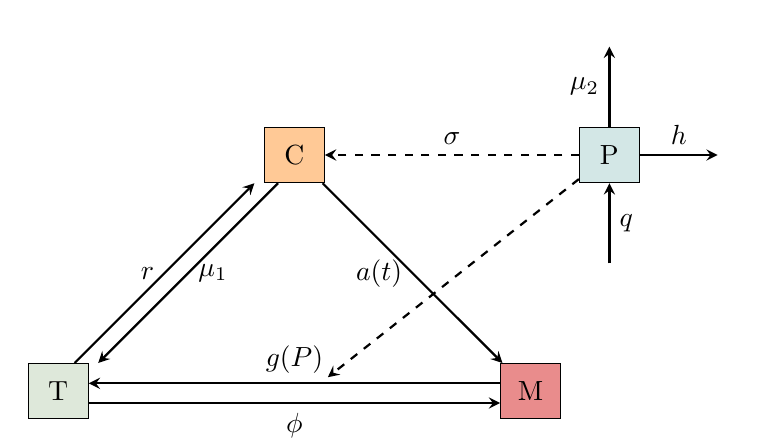
\begin{tikzpicture}{node distance = 1cm, auto}
        \node(leftofC) [noblock] {}; 
        \node(C) [block, right of = leftofC, node distance = 1.5 cm] {C};
        \node(P) [blockParrot, right of = C, node distance = 4 cm] {P};
        \node(belowofC) [noblock, below of = C, node distance = 3 cm]{};
        \node(M) [blockAlgae, right of = belowofC, node distance = 3 cm] {M};
        \node(T) [blockTurf, left of = belowofC, node distance = 3 cm] {T};
        \node(rightofP) [noblock, right of = P, node distance = 1.5 cm]{};
        \node(aboveofP) [noblock, above of = P, node distance = 1.5 cm]{};
        \node(aboveofC) [noblock, above of = C, node distance = 1.5 cm]{};
        \node(belowofP) [noblock, below of = P, node distance = 1.5 cm]{};
        \node(aboveofT) [noblock, above of = T, node distance = 0.08 cm]{};
        \node(diagonalofT) [noblock, right of = aboveofT, node distance = 3.3 cm]{};
        \draw[dline] (P) --node[above]{} (diagonalofT);
        \draw[dline] (P) --node[above]{$\sigma$} (C);
        \draw[line] (C) --node[left]{$a(t)$} (M);
        \draw[line] (P) --node[above]{$h$} (rightofP);
        \draw[line] (P) --node[left]{$\mu_{2}$} (aboveofP);
        %\draw[line] (C) --node[left]{$d$} (aboveofC);
        \draw[line] (belowofP) --node[right]{$q$} (P);
        \begin{scope}[transform canvas = {xshift = -.15cm}]
            \draw[line](T) -- node[left]{$r$} (C);
        \end{scope}
        \begin{scope}[transform canvas = {xshift = .15cm}]
            \draw[line](C) --node[right]{$\mu_{1}$} (T);     
        \end{scope}
        \begin{scope}[transform canvas = {yshift = .1cm}]
            \draw[line] (M) --node[above]{$g(P)$} (T);
        \end{scope}
        \begin{scope}[transform canvas = {yshift = -.15cm}]
            \draw[line] (T) --node[below]{$\phi$} (M);
        \end{scope}
        %\caption{Flowchart of coral reef ecosystem}
    \end{tikzpicture}
\end{center}

% assumptions and description of model
We assume that the (i) system is closed, (ii) it only consists of coral, macroalgae, and algal turfs, and (iii) macroalgae is the only predator for coral. Corals are assumed to (iv) recruit and overgrow algal turfs and that they are overgrown by macroalgae \textsuperscript{\cite{04_mathanalysis}}. Macroalgae are also assumed (v) colonize dead coral by spreading vegetative over algal turfs \textsuperscript{\cite{04_mathanalysis}}. In addition, (vi) corals do not die naturally and (vii) the maximum carrying capacity of parrotfish is equal to 1.

%Represented above is our general compartment model. While this version is a rough draft, it represents the compartments that we wish to include in our model. Included in our model is our $S$ compartment, which represents all susceptible corals, our $E$ compartment representing all exposed corals, our $I$ compartment representing our infected corals, and our $R$ compartment representing recovered corals. While this follows the standard SEIR model layout, we included an $H$ compartment to account for human factors. This is in order to assess how the human factor may directly or indirectly affect the typical "life" cycle of corals. \par
%The $H$ compartment allows to factor in the human factor to the overall equation, however in order to achieve this, we must implement education game theory. This is in order to model human factors such as education about corals, ignorance, and various other factors. By using education game theory, we are able to visualize which strategy is dominant between humans and corals, and reflect this strategy in our overall compartment model.

\subsection{Differential Equations}
C, T, and M are proportions of coral, algal turf, and macroalgae cover on the ocean floor, respectively,  where $C+M+T=1$ to signify the proportion of each population is a selected area. P is the population of the parrotfish that inhabit the coral reef ecosystem in proportion to the maximum carrying capacity. The coral reef dynamics are described as a system of nonlinear differential equations \textsuperscript{\cite{13_blackwood_hastings_mumby_2010}}: 
\begin{align*}
    \frac{dC}{dt} &= rTC + \sigma P C- (a(t)M+\mu_{1})C \label{eq:dCdt}\\
    \frac{dP}{dt} &= qP \left( 1-\frac{P}{\beta C} \right) - P \left( h+\mu_{2} \right) \label{eq:dPdt}\\
    \frac{dT}{dt} &= \mu_{1}C + \frac{g(P)M}{M+T} - T(rC+\phi M) \label{eq:dTdt}\\
    \frac{dM}{dt} &= (a(t)C+ \phi T)M - \frac{g(P)M}{M+T} \label{eq:dMdt}
\end{align*}

where: 
\begin{align*}
&g(P) = \frac{\omega P}{\beta}, a(t)=|\frac{a_{0}(9\sin{(\pi t) }+1)}{10}|\\
and\\
&\frac{g(P)M}{M + T} \text{ is the proportion of grazing that affects macroalgae} \textsuperscript{\cite{13_blackwood_hastings_mumby_2010}}.
\end{align*}

%See Table 1 for 

\subsection{Parameter Values}
\begin{table}[H]
    \centering
    \begin{tabular}{c p{9cm} c c}
        \hline
        Parameter & Description & Rate & Units\textsuperscript{\cite{12_noaa_report}\cite{04_mathanalysis}\cite{13_blackwood_hastings_mumby_2010}}\\
        \hline
        \hline
        $\mu_{1}$ & natural death rate of coral reefs & 0.15\textsuperscript{\cite{16_wolanski_richmond_mccook_2004}} & $year^{-1}$\\ %12
        $\mu_{2}$ & natural death rate of parrotfish & 0.22\textsuperscript{\cite{12_noaa_report}} & $year^{-1}$\\ %8
        $r$ & rate that coral recruit to overgrow algal turfs & 10\textsuperscript{\cite{16_wolanski_richmond_mccook_2004}} & $year^{-1}$\\ %12
        %$g$ & grazing rate that parrotfish graze macroalgae without distinction from algae turfs & $\frac{kg}{yrs}$\\
        $\phi$ & rate that macroalgae spread vegetative over algal turfs & 0.8\textsuperscript{\cite{11_zikkah_anggriani_supriatna_2020}} & $year^{-1}$\\ %13
        $q$ & intrinsic growth rate for parrotfish & 0.47\textsuperscript{\cite{12_noaa_report}} & $year^{-1}$\\ %8
        $h$ & harvesting rate for parrotfish & 0.14\textsuperscript{\cite{12_noaa_report}} & $year^{-1}$\\ %8
        $\sigma$ & rate that parrot fish bite coral & 0.01*& $bites*year^{-1}$\\
        $\omega$ & maximum grazing intensity & 1\textsuperscript{\cite{13_blackwood_hastings_mumby_2010}} & -\\
        $\beta$ & carrying capacity of parrotfish & 1 & -\\
        $a_{0}$ & control variable to simulate seasonal changes & 0.99 & - \\%13
        \hline
    \end{tabular}
    \caption{Model Parameters}
    \label{tab:parameters}
\end{table}
\textit{* = estimated values}

% graphs
\subsection{Graphs}
Using MatLab (See Appendix \ref{appendix:B1}), we were able to model the dynamics using our preliminary rates. This was achieved by changing the C, M, \& T proportions. Below are the graphs that were were able to achieve:\\
\begin{figure}[H]
    \centering
    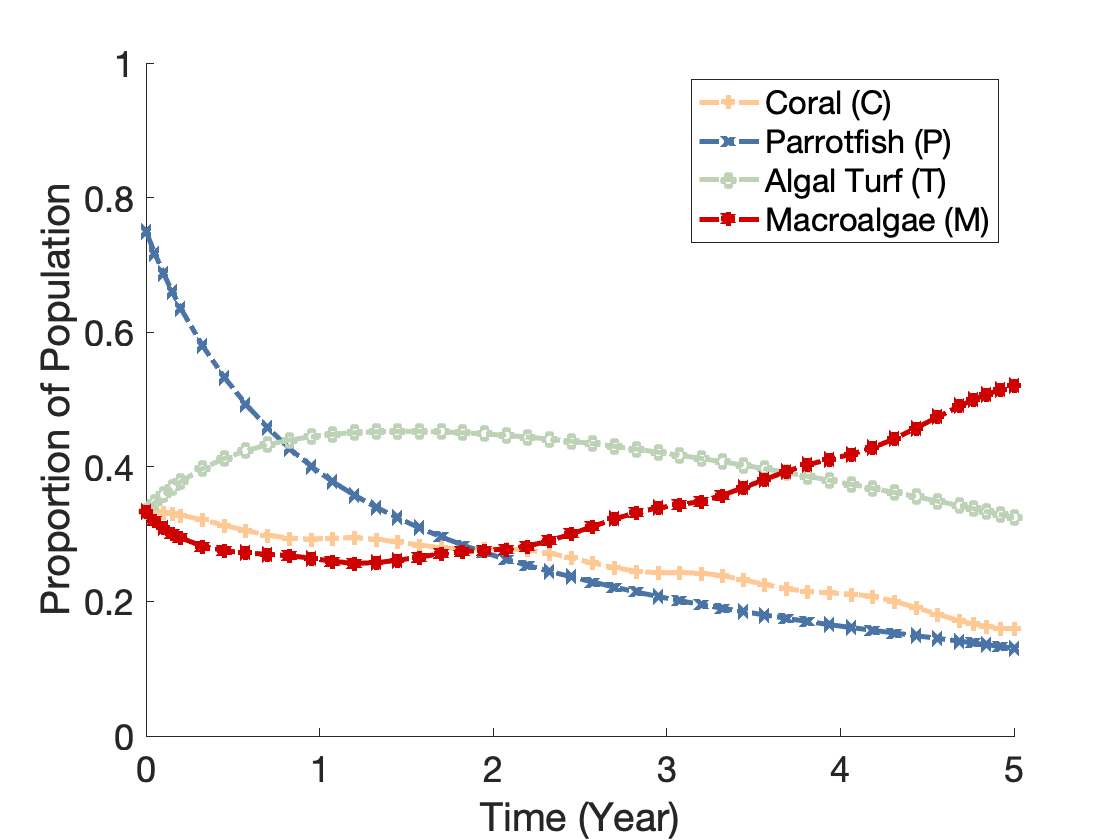
\includegraphics[width=0.7\textwidth]{Latex/Figures/Graphs/0.3C_0.3T_0.3M.png}
    \caption{Initial Conditions: $C = T = M = \frac{1}{3}$, and $P = \frac{3}{4}$}
    \label{fig:initial_plot}
\end{figure}
\begin{figure}[H]
    \centering
    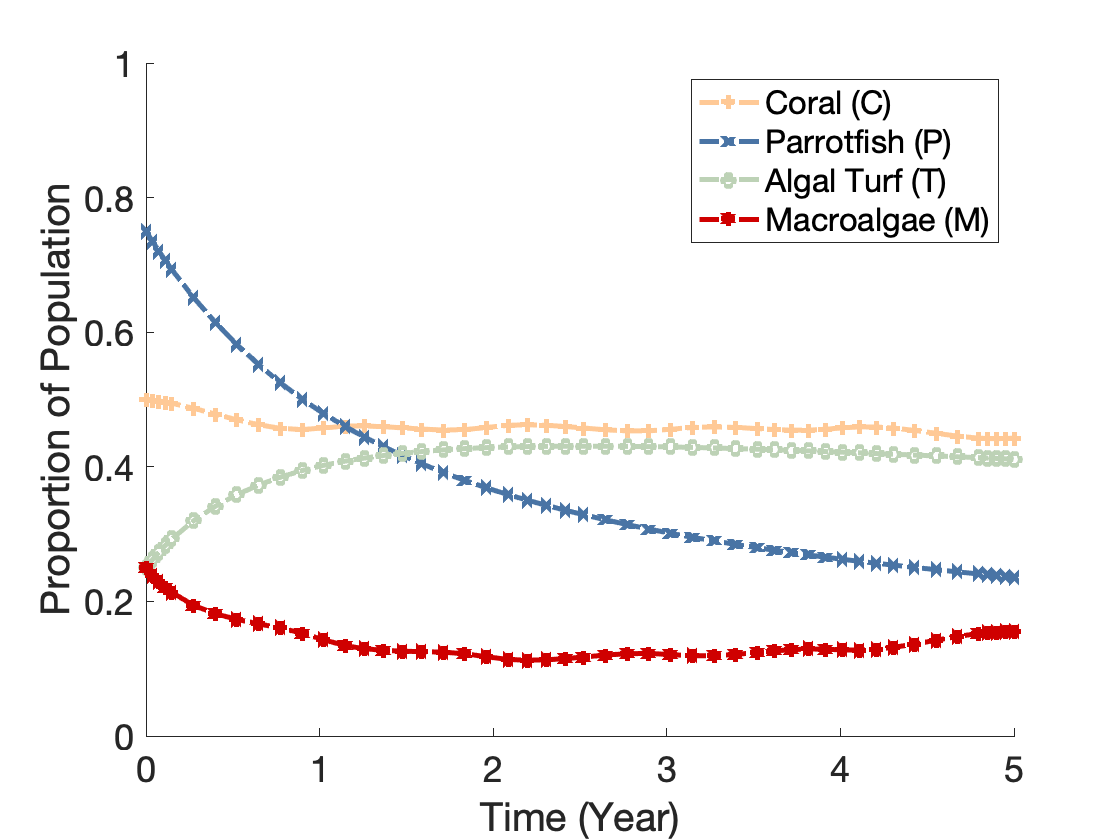
\includegraphics[width=0.7\textwidth]{Latex/Figures/Graphs/0.5C_0.25T_0.25M.png}
    \caption{Initial Conditions: $C = \frac{1}{2}$, $T = M = \frac{1}{4}$, and $P = \frac{3}{4}$}
    \label{fig:coral_dominant}
\end{figure}
\begin{figure}[H]
    \centering
    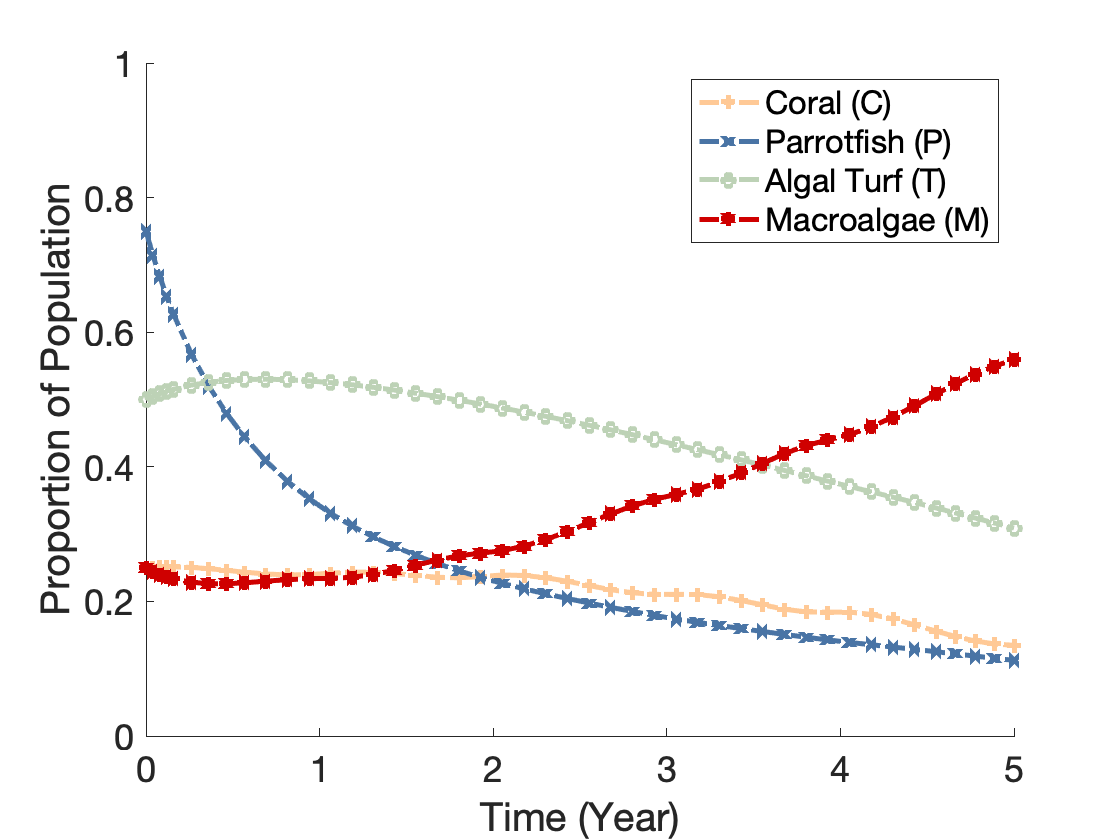
\includegraphics[width=0.7\textwidth]{Latex/Figures/Graphs/0.25C_0.5T_0.25M.png}
    \caption{Initial Conditions: $T = \frac{1}{2}$, $C = M = \frac{1}{4}$, and $P = \frac{3}{4}$}
    \label{fig:turf_dominant}
\end{figure}
\begin{figure}[H]
    \centering
    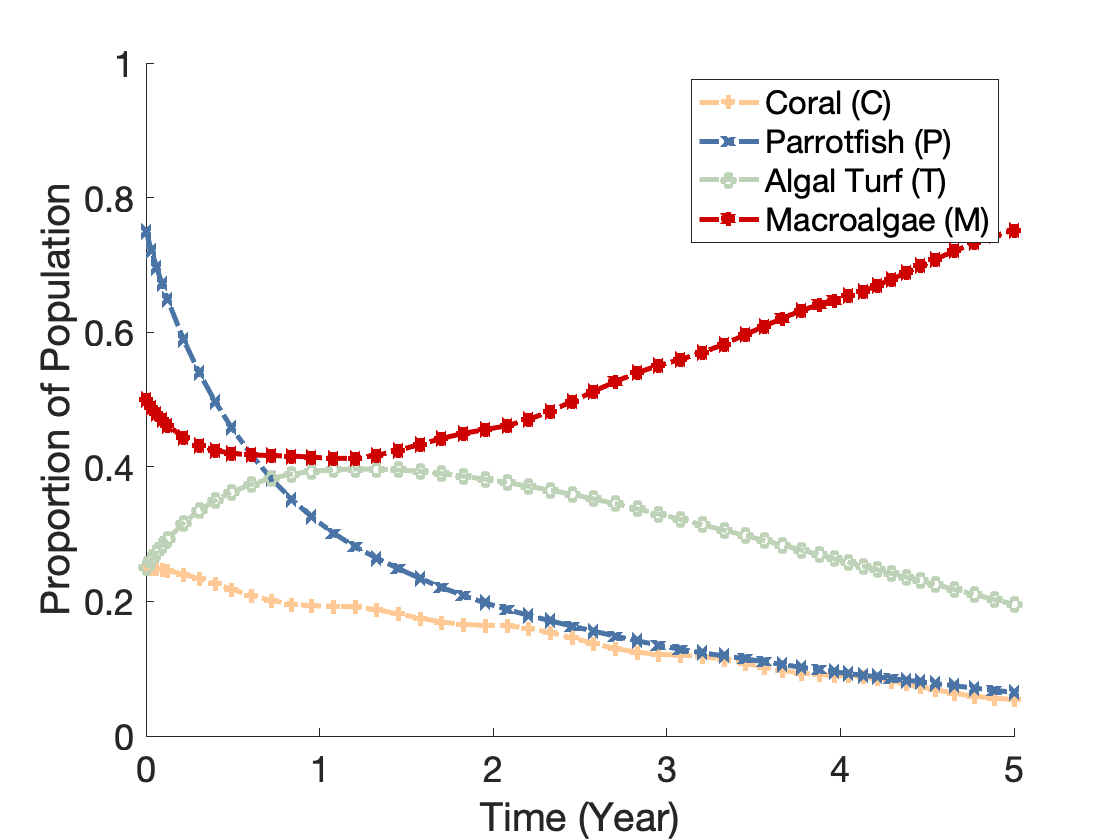
\includegraphics[width=0.7\textwidth]{Latex/Figures/Graphs/0.25C_0.25T_0.5M.png}
    \caption{Initial Conditions: $M = \frac{1}{2}$, $C = T = \frac{1}{4}$, and $P = \frac{3}{4}$}
    \label{fig:macroalgae_dominant}
\end{figure}
As we can see in Figures \ref{fig:initial_plot}, \ref{fig:coral_dominant}, \ref{fig:turf_dominant}, \& \ref{fig:macroalgae_dominant}, as the parrot fish population decreases, the macroalgae proportion increases. In addition, as the macroalgae proportion increases, the coral proportion decreases, and subsequently the algal turf proportion decreases as well.\\

\section{Equilibria Analysis}
\subsection{Disease-Free Equilibrium}
The disease-free equilibrium, or DFE, is the point at which no disease is present in the system. Typically, this method is performed on disease modeling, however can be adapted to other types of modeling as well. In our model, we classify macroalgae (M) as our "disease" compartment, and since the system is disease free, we set $M^{0} = 0$. Below is the result of our DFE calculations (detailed in Appendix \ref{appendix:A1}):
\begin{align*}
        C^{0} &= 1 - \frac{\mu_{1}}{r} \label{eq:C0}\\
        P^{0} &= -\frac{\beta(1 - \frac{\mu_{1}}{r})(h - \mu_{2} - q)}{q} \label{eq:P0}\\
        T^{0} &= \frac{\mu_{1}}{r} \label{eq:T0}\\
        M^{0} &= 0 \label{eq:M0}
\end{align*}
Since our model was set-up so as $C+T+M=1$ and since $M^{0} = 0$, then we conclude that $C^{0} + T^{0} = 1$. Thus, our disease-free equilibrium is $(1 - \frac{\mu_{1}}{r}, -\frac{\beta(1 - \frac{\mu_{1}}{r})(h - \mu_{2} - q)}{q}, 0, \frac{\mu_{1}}{r})$.

\subsection{Basic Reproduction Number: $\mathscr{R}_{0}$}
The basic reproduction number, $\mathscr{R}_{0}$, is a metric used to describe the contagiousness or transmissibility of infectious agents\textsuperscript{\cite{delamater_street_leslie_yang_jacobsen_2019}}. In essence, this equation measures the number of secondary infections. Since our model is not disease-based, we conclude that our $\mathscr{R}_{0}$ symbolizes the rate at which macroalgae spreads after the initial macroalgae overgrowth. Our model recognizes macroalgae (M) as our infectious compartment. By using our disease-free equilibrium equations, we are able to calculate our $\mathscr{R}_{0}$ equation (detailed in Appendix \ref{appendix:A3}): 
\begin{equation*}\label{eq:R0}
    \displaystyle {\mathscr{R}}_{0} = - \frac{\beta \mu_{1}q(a(t)(\frac{\mu_{1}}{r}-1)-\frac{\mu_{1}}{r})}{\omega r (\beta h (\frac{\mu_{1}}{r}-1) + \beta \mu_{2} (\frac{\mu_{1}}{r}-1) - \beta q(\frac{\mu_{1}}{r}-1))}
\end{equation*}

\subsection{Endemic Equilibrium}
The Endemic Equilibrium determines at what point will the disease not spread nor will it fully eradicate. Essentially it tells when the disease is stabilized. In order to find the endemic equilibrium, we have to set each differential equal to 0 and solve for each variable. The equations above are in terms of M as M is considered our disease, as shown below (detailed in Appendix \ref{appendix:A2}):
\begin{align*}
        T^{*} &= \frac{\mu_{1} + a(t)M^{*}}{r} \label{eq:T*}\\
        C^{*} %&= 1-(T^{*} + M^{*}) \\
        &= 1- \left(\frac{\mu_{1} + a(t)M^{*}}{r} + M^{*} \right) \label{eq:C*}\\
        P^{*} %&= \beta C^{*} \left(\frac{q-(h+\mu_{2})}{q} \right) \\
        &= \beta \left(1- \left(\frac{\mu_{1} + a(t)M^{*}}{r} + M^{*} \right) \right) \left(\frac{q-(h+\mu_{2})}{q} \right) \label{eq:P*}\\
        M^{*} &= \frac{\omega (\beta \left(1- \left(\frac{\mu_{1} + a(t)M^{*}}{r} + M^{*} \right) \right) \left(\frac{q-(h+\mu_{2})}{q} \right))}{\beta(a(t)(1- \left(\frac{\mu_{1} + a(t)M^{*}}{r} + M^{*}) \right)+\phi \frac{\mu_{1} + a(t)M^{*}}{r})} - \frac{\mu_{1} + a(t)M^{*}}{r} \label{eq:M*}
\end{align*}

While not a disease model, the endemic equilibrium equations are significant in our research project as it is essential in order to perform game theory on our model. 

\subsection{Sensitivity Analysis}
Sensitivity analysis determines the maximum impact of each parameter on the basic reproduction number equation. This process is calculated by performing the partial derivative on the $\mathscr{R}_0$ equation(\ref{eq:R0}) with respect to each parameter value, and substituting the values for the remaining parameter variables. Below is the general equation to calculate sensitivity analysis: \\
\begin{equation*}\label{eq:sens_analysis}
        S_{\lambda} = \frac{\frac{\Delta \mathscr{R}_{0}}{\mathscr{R}_{0}}}{\frac{\Delta x}{x}} = \frac{\lambda}{\mathscr{R}_{0}} \cdot \frac{\partial \mathscr{R}_{0}}{\partial \lambda}
\end{equation*}
\begin{center}
    where $\lambda$ is a parameter in the quantity $\mathscr{R}_{0}$
\end{center}
%where $\lambda$ is a parameter in the quantity $\mathscr{R}_{0}$.

Utilizing MatLab (Appendix \ref{appendix:B6}), we were able to automate the calculation process, giving us the corresponding sensitivity analysis for each parameter variable. 
\begin{table}[H]
        \centering
        \begin{tabular}{|c|c|}
            \hline
            Parameter & $S_{A}$ \\
            \hline
            \hline
            $\mu_{1}$ & \colorbox{yellow}{\textbf{8.3513}}\\
            \hline
            $\mu_{2}$ & \colorbox{yellow}{\textbf{5.2819}}\\
            \hline
            $q$ & -3.5962\\
            \hline
            $\omega$ & -0.7923\\
            \hline
            $\sigma$ & 0.0000\\
            \hline
            $r$ & -2.5054\\
            \hline
            $\phi$ & 0.4029\\
            \hline
            $\beta$ & 0.0000\\
            \hline
            $h$ & \colorbox{yellow}{\textbf{5.2819}}\\
            \hline
            $a$ & 0.9400\\
            \hline
        \end{tabular}
        \caption{Sensitivity Analysis}
        \label{tab:sens_analysis}
    \end{table}
    
    The larger the sensitivity analysis value, the higher the impact the parameter has on our basic reproduction number equation. The highlighted values ($\mu_{1}, \mu_{2}$, and $h$) have the largest sensitivity analysis values, and have the most impact on our basic reproduction number equation, respectively. \par
    The natural death rate of corals ($\mu_{1}$) represents the largest impact, and rightfully so, with a sensitivity analysis value of 8.3513. Due to the dynamics between corals, algal turfs, and macroalgae, the death of corals directly impacts algal turfs. However, the natural death accounts for all factors of coral deaths, including but not limited to bleaching, disease, damage, and so forth. The more corals that die, the more surface area get converted into algal turfs and subsequently gives way for algal turfs to convert into macroalgae. As such, this rate carries the greatest impact on our overall basic reproduction number equation. \par
    The natural death rate of parrotfish ($\mu_{2}$) and the harvest rate of parrotfish due to fishing ($h$) both share the second highest sensitivity analysis value of 5.2819. This presents a unique perspective, as the analysis indicates that there is no difference between natural death and hu1man-driven death. Both simply represent the removal of live parrotfish from the ecosystem rather than the means of removal, and as such are equal. This is significant as our model depicts parrotfish as the primary grazers of macroalgae, and we have acknowledged that macroalgae overgrowth has a negative impact on the ecosystem. When the parrotfish population is adequate, the proportion of macroalgae will be kept in control. However, with the removal of parrotfish from the ecosystem from death or fishing, the macroalgae will have the opportunity to grow unchecked. Thus, the impact of overfishing parrotfish will undeniably affect the dynamics of the ecosystem, and will allow macroalgae to dominate while corals whither away.
    
\section{Harvesting Game Theory}
One of the primary objectives of our research is to implement game theory to our project. Game theory is essentially "a theoretical framework to conceive social situations among competing players and produce optimal decision-making of independent and competing actors in a strategic setting."\textsuperscript{\cite{game_theory_definition}}. By taking into account strategies, we can apply game theory to predict outcomes. \par
In our project, we apply education game theory to our $h$ parameter, or the harvest rate of parrotfish. Our goal is to best predict an individual's choice towards the harvesting of parrotfish in response to the population's choice towards the harvesting of parrotfish. As such, we adapt the concept of education game theory and apply it to our Game of Harvesting. 

\subsection{Harvesting Threshold}
The first step in performing game theory is isolating our parameter, in this case $h$, from our basic reproduction number equation (\ref{eq:R0}). By isolating our parameter when $\mathscr{R}_0 = 1$, we are able to find our harvesting threshold, which is the rate at which parrotfish can be harvested in order for macroalgae growth to become stable in the ecosystem:\\
\\
When $\mathscr{R}_{0} = 1$,
\begin{equation*}\label{eq:h_TH}
    \displaystyle{h_{TH} = q - \mu_{2} + \frac{\mu_{1}q(a(t) \mu_{1} - a(t)r - \phi \mu_{1})}{\omega r(r-\mu_{1})}}
\end{equation*}
Furthermore, we are able to plot our harvesting threshold against our $\mathscr{R}_{0}$ equation, giving us the figure below.
\begin{figure}[H]
    \centering
    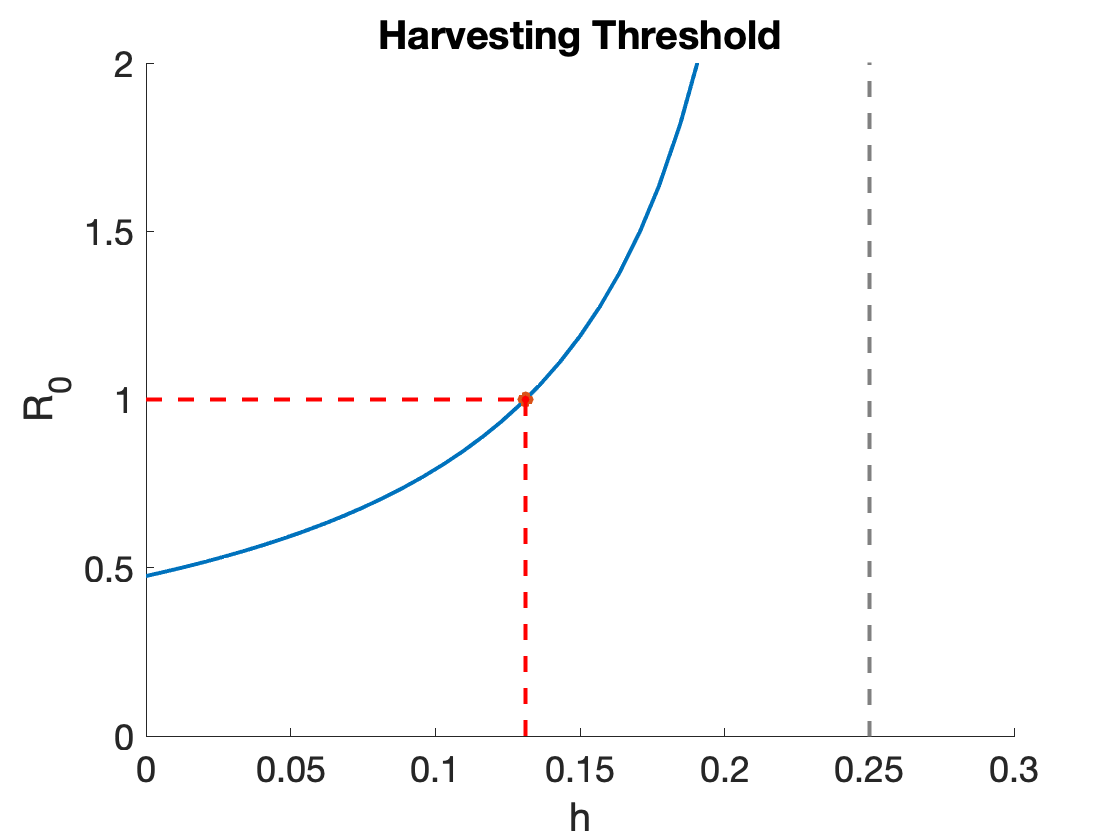
\includegraphics[width=0.8\textwidth]{Latex/Figures/Graphs/threshold_graph.png}
    \caption{Threshold Analysis}
    \label{fig:threshold_graph}
\end{figure}
We can see from Figure \ref{fig:threshold_graph} that when $\mathscr{R}_{0} = 1$, $h=0.1312$. This point represents our threshold. According to Drieche and Wattmough\textsuperscript{\cite{bible}}, any point ($h$ value) above the threshold will result in an unstable system, and any point ($h$ value) below the threshold will be stable.
\begin{align*}
    h_{pop} &< h_{TH}: \text{Macroalgae growth is stable} \\
    h_{pop} &> h_{TH}: \text{Macroalgae growth is unstable}
\end{align*}

\subsection{Expected Payoff}
In terms of game theory, an expected payoff is an equation representing the benefit of the player's decision. In our game, expected payoff is the proportion at which an individual can harvest parrotfish. As such, we create the following expected payoff equation based on our compartment model:
\begin{equation*}\label{eq:initial_payoff}
    \displaystyle {E(h, h_{pop}) = -hC_{h} - \left( \frac{h_{pop}}{h_{pop} + \mu_{2}} \cdot \frac{g(P^{*})(1-h)M^{*}}{M^{*} + T^{*}} \right) C_{D}}
\end{equation*}
where
\begin{table}[H]
    \centering
    \begin{tabular}{c|p{9cm}}
         Symbol & Definition \\
         \hline
         $E(h, h_{pop})$ & Expected payoff for an individual to harvest based on the harvesting rate of the population \\
         $C_{h}$ & Cost of harvesting \\
         $C_{D}$ & Cost of coral disease \\
    \end{tabular}
    %\caption{Caption}
    \label{tab:payoff_eq_params}
\end{table}
and $h \in [0,1]$. \\
We can further simplify by dividing the equation by $C_{D}$, giving us 
\begin{equation*}\label{eq:payoff}
    \displaystyle {E(h, h_{pop}) = -hC^{h} - \frac{h_{pop}}{h_{pop} + \mu_{2}} \cdot \frac{g(P^{*})(1-h)M^{*}}{M^{*} + T^{*}}}
\end{equation*}
where $C^{h} = \frac{C_{h}}{C_{D}}$. \\ \par
In order to confirm that a Nash equilibrium exists for our expected payoff equation (\ref{eq:payoff}), we must find the second partial derivative of our expected payoff equation with respect to $h$. If $\frac{\partial^{2}E(h, h_{pop})}{\partial h^{2}} > 0$, then we can confirm through the convex function that $E$ achieves a maximum value at $h=0$ and $h=1$. \par
\begin{equation*}\label{eq:nash_partial_deriv}
    \displaystyle {\frac{\partial ^ {2} E}{\partial h^{2}} = \frac{2 \omega P^{*} \mu{2} (M^{*}+T^{*})^{2} (\mu_{1} +1)}{\beta(h(M^{*}+T^{*}) + \mu_{2}(M^{*}+T^{*}))^{3}} > 0}
\end{equation*}
We find that the second partial derivative of our expected payoff equation with respect to $h$ is indeed greater than 0, and thus a valid solution.

\subsection{Nash Equilibrium}
The Nash equilibrium, named after mathematician John Nash, is a decision-making theorem within game theory that states a player can achieve the desired outcome by not deviating from their initial strategy, and thus, each player's strategy is optimal when considering the decision of other players\textsuperscript{\cite{nash_definition}}. \par
In the case of our harvesting game theory, we can obtain the Nash equilibrium by setting our payoff equations equal to each other:
\begin{equation*}
    E(0, h_{pop}) = E(1, h_{pop})
\end{equation*}
By substituting in $E(0, h_{pop})$ and $E(1, h_{pop})$, we create the following equation:
\begin{equation*}\label{eq:unsimplified_nash}
    \frac{h_{pop}}{h_{pop} + \mu_{2}} \cdot \frac{g(P^{*})(1-h)M^{*}}{M^{*} + T^{*}} = C^{h}
\end{equation*}

\section{Conclusion}


%\section{Literature Review}
%Throughout this week, our group has dedicated a large portion of time to reviewing scholarly articles and research publications relevant to our areas of research. This aspect of performing our research is crucial as, through literature review, we are able to gather information, techniques, methods, data, results, and many other variables that we are able to use in our own research. \par
%Our faculty mentors have graciously provided several research publications related to the overall study coral reef ecosystems in order to stimulate creativity in creating our own research topic. These papers are as follow:
%\begin{itemize}
    %\item Assessing relative resilience potential of coral reefs to inform management\textsuperscript{\cite{01_assesing_relative}}
    %\item Model of coral population response to accelerated bleaching and mass mortality in a changing climate\textsuperscript{\cite{02_Riegl_Purkis_Model}}
    %\item Prioritizing Key Resilience Indicators to Support Coral Reef Management in a Changing Climate\textsuperscript{\cite{03_prioritize}}
    %\item Mathematical analysis of coral reef models\textsuperscript{\cite{04_mathanalysis}}
    %\item A Mathematical Model of Coral Reef Response to Destructive Fishing Practices with Predator-Prey Interactions\textsuperscript{\cite{05_quintero_machuca_cotto_bradley_ríos-soto_2016}}
    %\item From bee species aggregation to models of disease avoidance: The Ben-Hur effect\textsuperscript{\cite{06_yong_herrera_castillo-chavez_2016}}
    %\item Vaccination and the theory of games\textsuperscript{\cite{07_bauch_earn_2004}}
    %\item The effect of fishing on hysteresis in Caribbean coral reefs \textsuperscript{\cite{13_blackwood_hastings_mumby_2010}}
%\end{itemize}
%These articles provide valuable insight in various areas of coral reef research from parameters and conditions to modeling and application. In particular, each of these papers gave us insight on how other researchers approached their problems, how they created and modified their methods, and how they produced results based on their models and equations. 

\section{Acknowledgements}
Support for the Young Scholars Research Experience in Mathematics (YSREM)  is through the MAA Tensor SUMMA Program. Support for the MAA National Research Experience for Undergraduates Program (NREUP) is provided by the National Science Foundation (Grant Number DMS-1950644). Support for the NSF EPSCoR project, Guam Ecosystems Collaboratorium for Corals and Oceans (GECCO) is provided by the National Science Foundation (Grant Number DMS-1946352). \par
Special thanks to Dr. Bastian Bentlage, our faculty mentors (Dr. JaeYong Choi, Dr. HyunJu Oh, \& Dr. Leslie Aquino), and our Research Assistants (Jaron Bautista \& Regina-Mae Dominguez).

\newpage
\appendix
    {\huge \textbf{Appendix}}
    \section{Step-by-Step Calculations}
    \subsection{Disease Free Equilibrium}
        \label{appendix:A1}
        The disease-free equilibrium occurs when we have $(C, M, T, P) = (C^{0}, 0, T^{0}, P^{0})$. 

        Solving for $T^{0}$, let $\frac{dT}{dt} = 0$: 
            \begin{align*}
                0 &= \mu_{1}C^{0} + \frac{g(P)M^{0}}{M^{0} + T^{0}} - T(rC^{0} + \phi M^{0}) \\
                rC^{0}T^{0} &= \mu_{1}C^{0} \\
                T^{0} &= \frac{\mu_{1}}{r} \\
            \end{align*}
            
        Solving for $P^{0}$, let $\frac{dP}{dt} = 0$:
            \begin{align*}
                0 &= qP^{0} \left( 1-\frac{P^{0}}{\beta C^{0}}\right) - P^{0}(h + \mu_{2}) \\
                0 &= P\left( q\left(1- \frac{P^{0}}{\beta C^{0}} \right) - h - \mu_{2} \right) \\
                0 &= q - \frac{qP^{0}}{\beta C^{0}} - h - \mu_{2} \\
                -\frac{qP^{0}}{\beta C^{0}} &= h + \mu_{2} -q \\
                qP^{0} &= -\beta C^{0}(h + \mu_{2} - q) \\
                P^{0} &= \frac{-\beta C^{0}(h + \mu_{2} - q)}{q}
            \end{align*}
            
        Solving for $C^{0}$, let $\frac{dC}{dt} = 0$: \\ \par
        Since $C + M + T = 1$, then
            \begin{align*}
                C^{0} + M^{0} + T^{0} &= 1 \\
                C^{0} + T^{0} &= 1 \\
                C^{0}  &= 1 - T^{0} \\
                &= 1 - \frac{\mu_{1}}{r}
            \end{align*}
            
        After inputting $C^{0}$ into $P^{0}$, we obtain the disease free equilibrium at \\
        \begin{center}
        $\displaystyle{(C^{0}, M^{0}, T^{0}, P^{0}) = \left(1 - \frac{\mu_{1}}{r}, 0, \frac{\mu_{1}}{r}, -\frac{\beta(1 - \frac{\mu_{1}}{r})(h - \mu_{2} - q)}{q }\right)}$. 
        \end{center}
        
    \subsection{Endemic Equilibrium}
        \label{appendix:A2}
        First, we solved each differential equation in terms of M: \\ \\
        \begin{itemize}
            \item Calculating $T^{*}$ :
                \begin{align*}
                    \frac{dT}{dt} &= \mu_{1}C + \frac{g(P)M}{M+T} - T(rC+\phi M) \\
                    0 &= \mu_{1}C + \frac{g(P)M}{M+T} - T(rC+\phi M) \\
                    0 &= \mu_{1}C + \frac{g(P)M}{M+T} - rTC+\phi TM) 
                \end{align*}
                The term $\phi TM$ cancel out with the similar term from the $\frac{dM}{dt}$ equation (\ref{eq:dMdt}). Thus, we are left with:
                \begin{align*}
                    0 &= \mu_{1}C + a(t)MC - rTC \\
                    rTC &= \mu_{1}C + a(t)MC \\
                    T &= \frac{\mu_{1} + a(t)M}{r}
                \end{align*}
                Solving for T when $\frac{dT}{dt} = 0$, we have:
                \begin{equation*}
                    T^{*} = \frac{\mu_{1} + a(t)M^{*}}{r}
                \end{equation*}
            \item Calculating $C^{*}$ :
                Since $C^{*}+T^{*}+M^{*} = 1$, then
                \begin{equation*}
                    \frac{dC}{dt} = 1 - T^{*} - M^{*} 
                \end{equation*}
                Having already solved for $T^{*}$, we are able to substitute in $T^{*}$ to find $C^{*}$:
                \begin{equation*}
                    \frac{dC}{dt} = 1 - \frac{\mu_{1} + a(t)M^{*}}{r} - M^{*} 
                \end{equation*}
            \item Calculating $P^{*}$ :
                \begin{align*}
                    \frac{dP}{dT} &= qP\left(1-\frac{P}{\beta C}\right) - P(h + \mu_{2})\\
                    0 &= qP\left(1-\frac{P}{\beta C}\right) - P(h + \mu_{2})\\
                    P(h+ \mu_{2}) &= qP\left(1-\frac{P}{\beta C}\right)\\
                    \frac{(h+ \mu_{2})}{q} &= \left(1-\frac{P}{\beta C}\right)\\
                    \frac{P}{\beta} C &= 1 - \frac{h+\mu_{2}}{q}\\
                    P^{*} &= \beta C^{*} \left(\frac{q-(h+\mu_{2})}{q}\right)
                \end{align*}
                Having already solved for $C^{*}$, we are able to substitute in $C^{*}$ to find $P^{*}$ in terms of $M^{*}$: 
                \begin{equation*}
                    P^{*} = \beta \left(1- \left(\frac{\mu_{1} + a(t)M^{*}}{r} + M^{*} \right) \right) \left(\frac{q-(h+\mu_{2})}{q} \right)
                \end{equation*}
            \item Calculating $M^{*}$ :
                \begin{align*}
                    \frac{dM}{dt} &= (a(t)C+ \phi T)M - \frac{g(P)M}{M+T} \\
                    0 &= a(t)CM+ \phi TM - \frac{g(P)M}{M+T} \\
                    0 &= a(t)CM+ \phi TM - \frac{\frac{\omega P}{\beta}M}{M+T} \\
                    0 &= a(t)CM+ \phi TM - \frac{\omega PM}{\beta(M+T)} \\
                    0 &= a(t)CM\beta(M+T)+ \phi TM\beta(M+T) - \omega PM \\
                    M &= \frac{\omega P}{\beta(a(t)C+\phi T)} - T
                \end{align*}
                Thus, we find that $M^{*}$ is
                \begin{equation*}
                    M^{*} = \frac{\omega P^{*}}{\beta(a(t)C^{*}+\phi T^{*})} - T^{*}
                \end{equation*}
        \end{itemize}
        
    By substituting all our $E^{*}$ equations into $M^{*}$ (i.e. $P^{*}$, $T^{*}$, and $C^{*}$), we are able to find an equation in terms of parameters, which can then be substituted into calculate a value. So, we get
    \begin{align*}
        M^{*} &= \frac{\beta \omega(1-\frac{\mu_{1} + a(t)M^{*}}{r}-M^{*})(q - h - \mu_{2})}{\beta q (\frac{a(t)(r-\mu_{1}-a(t)M^{*}-rM^{*}}{r}) + \frac{\phi(\mu_{1} + a(t)M^{*})}{r})} - \frac{\mu_{1} + a(t)M^{*}}{r} \\
        &= \frac{\omega(1-\frac{\mu_{1} + a(t)M^{*}}{r}-M^{*})(q - h - \mu_{2})}{q (\frac{a(t)(r-\mu_{1}-a(t)M^{*}-rM^{*}}{r}) + \frac{\phi(\mu_{1} + a(t)M^{*})}{r}} - \frac{\mu_{1} + a(t)M^{*}}{r} \\
        &= \frac{r\omega (q-h-\mu_{2})((r-\mu_{1})-(a(t) + r)M^{*} - (\mu_{1} + a(t)M^{*}q((a(t)r - a \mu_{1} + \phi \mu_{1}) + (-(a(t))^{2} - a(t)r + \phi a(t))M^{*})}{rq((a(t)r - a(t) \mu_{1} + \phi \mu_{1}) + (-(a(t))^{2} - a(t)r + \phi a(t))M^{*})} \\
    \end{align*}
    
    % idk how to make this part look better
    \begin{center}
        $rq(a(t)r-a(t)\mu_{1} + \phi \mu_{1})M^{*} + rq(-(a(t))^{2} - a(t)r + \phi a(t))(M^{*})^{2} = r \omega (q - h - \mu_{2})(r - \mu_{1}) - r \omega(q-h-\mu_{2})(a(t)+r)M^{*} - q \mu_{1}(a(t)r-a(t) \mu_{1} + \phi \mu_{1}) - q(a(t)(a(t)r-a(t) \mu_{1} + \phi \mu_{1}) + \mu_{1}(-(a(t))^{2}-a(t)r+\phi a(t)))M^{*} - a(t)q(-a^{2}-a(t)r+ \phi a(t))(M^{*})^{2}$ \\ 
    \end{center}
    
    By isolating all $M^{*}$ terms on one side, we obtain
    \begin{align*}
        (M^{*})^{2}&[a(t)q(a+r)(-a(t)-r+\phi)] +  \\ 
        M^{*}&[q(a(t) - a(t) \mu_{1} + \phi \mu_{1})(a(t) + r) + r \omega (q-h-\mu_{2})(a(t) +r)] +  \\
        &[-r \omega(q - h - \mu_{2})(r - \mu_{1}) + q \mu_{1}(a(t)r - a(t) \mu_{1} + \phi \mu_{1}] \\
        &= 0
    \end{align*}
    
    %and performing algebraic simplification, 
    
    Thus, the general equation of $M^{*}$ is
    \begin{align*}
        d &= (a(t)q-2a(t)r+r \phi ) - q(r^{2}+a(t)^{3})\\
        e &= a(t)q(r(r-2\mu_{1}+a(t))-2\mu_{1}(a(t)+\phi )) +  r(q(\phi \mu_{1} + r \omega ) - \\ & \ \ \  \omega(hr+a(t) \mu_{2} + r\mu_{2})\\
        f &= -qr^{2} \omega +qr\mu_{1} \omega + hr^{2} \omega - hr\mu_{1} \omega + r^2 \mu_{2} \omega - r \mu_{1} \mu_{2} \omega + a(t)qr \mu_{1} - \\ & \ \ \  a(t)q\mu_{1}^{2} +q\phi \mu_{1}^{2}
    \end{align*}
    where $d$, $e$, and $f$ are values in the general quadratic equation:
    $$\frac{-e \pm \sqrt{e^2 - 4df}}{2d}$$

    \subsection{Basic Reproduction Number: $\mathscr{R}_0$}
        \label{appendix:A3}
        Firstly, we will set-up our $\mathscr{F}$ and $\mathscr{V}$ matrices, which are:
        \begin{align*}
            \mathscr{F} &= \begin{bmatrix}
                            a(t)CM + \phi MT
                          \end{bmatrix}\\
            \mathscr{V} &= \begin{bmatrix}
                            \frac{g(P)M}{M+T}
                          \end{bmatrix}              
        \end{align*}
        
        Since $M$ is considered our infected compartments, we will find the partial derivatives with regards to $M$ using Jacobian Matrices:
        $$\mathscr{F} = \begin{bmatrix}
                            aCM + \phi MT
                        \end{bmatrix}
            \longrightarrow
            F = \begin{bmatrix}
                a(t)C^{0} + \phi T^{0}
            \end{bmatrix}
        $$
        $$\mathscr{V} = \begin{bmatrix}
                            \frac{g(P)M}{M+T}
                        \end{bmatrix}
                        \longrightarrow
          V = \begin{bmatrix}
                \frac{g(P)T^{0}}{(M^{0}+T^{0})^{2}}
              \end{bmatrix}
        $$\\
        (Note: Since we are simply using a 1 $\times$ 1 $\mathscr{F}$ and $\mathscr{V}$, performing a Jacobian matrix operation is equivalent to performing a single partial derivative operation with respect to $M$.)
        After calculating for $F$ and $V$, we will calculate the inverse of $V$ by taking the reciprocal of $V$:
        $$V = \begin{bmatrix}
                \frac{g(P)T^{0}}{(M^{0}+T^{0})^{2}}
              \end{bmatrix}
          \longrightarrow
          V^{-1} = \begin{bmatrix}
                    \frac{aC^{0}T^{0} + \phi (T^{0})^{2}}{g(P^{0})}
                  \end{bmatrix}
        $$
        Our next step is to calculate $FV^{-1}$, which is found by matrix multiplication:
        \begin{align*}
            FV^{-1} &=\begin{bmatrix}
                            a(t)C^{0} + \phi T^{0}
                        \end{bmatrix}
                        \cdot
                        \begin{bmatrix}
                            \frac{aC^{0}T^{0} + \phi (T^{0})^{2}}{g(P^{0})}
                        \end{bmatrix} 
                    \\
                    &= \begin{bmatrix}
                            \frac{(a(t)C^{0}T^{0}+\phi (T^{0})^{2})(a(t)C^{0}T^{0})}{g(P^{0})}
                        \end{bmatrix}
        \end{align*}
        
        Lastly, we are able to calculate the eigenvalues of our $FV^{1}$ result:
        \begin{align*}
            \det(FV^{-1} - \lambda I) &= \begin{bmatrix}
                                            \frac{(a(t)C^{0}T^{0}+\phi (T^{0})^{2})(a(t)C^{0}T^{0})}{g(P^{0})}
                                        \end{bmatrix}
                                        - \lambda
                                        \begin{bmatrix}
                                            1 
                                        \end{bmatrix}
                                    \\
                                    &= \begin{bmatrix}
                                            \frac{(a(t)C^{0}T^{0}+\phi (T^{0})^{2})(a(t)C^{0}T^{0})}{g(P^{0})} - \lambda 
                                        \end{bmatrix}
                                    \\
                                    &= \frac{(a(t)C^{0}T^{0}+\phi (T^{0})^{2})(a(t)C^{0}T^{0})}{g(P^{0})} - \lambda
        \end{align*}
        
        To calculate the eigenvalues, we must set the solution of $\det(FV^{-1} - \lambda I) = 0$, which gives us:
        \begin{equation*}
            \lambda = -\frac{(a(t)C^{0}T^{0}+\phi (T^{0})^{2})(a(t)C^{0}T^{0})}{g(P^{0})}
        \end{equation*}
        Typically, $\mathscr{R}_{0}$ will be the largest of all eigenvalues, however since we only have one eigenvalue, the singular eigenvalue will be our $\mathscr{R}_{0}$. After substituting in $C^{0}$, $T^{0}$, and $P^{0}$, our $\mathscr{R}_{0}$ is
        \begin{equation*}
            \displaystyle {\mathscr{R}}_{0} = - \frac{\beta \mu_{1}q(a(t)(\frac{\mu_{1}}{r}-1)-\frac{\mu_{1}}{r})}{\omega r (\beta h (\frac{\mu_{1}}{r}-1) + \beta \mu_{2} (\frac{\mu_{1}}{r}-1) - \beta q(\frac{\mu_{1}}{r}-1))}
        \end{equation*}


    %\subsection{Harvesting Game Theory}
        %\label{appendix:A4}
    %Expected Payoff: 
    %\begin{align*}
        %E (h, h_{pop}) &= -hC^{h} - \frac{h}{h+\mu_{2}} \frac{g(P)(1-h)M}{M+T}
    %\end{align*}
    
    \section{MatLab Scripts}
        \subsection{Static Compartment Model Visualization}
        \label{appendix:B1}
        This script represents our MatLab implementation of visualizing our compartment model and dynamics using our known and estimated parameters. The code implements ODE45 in order to calculate our system of differential equations, and plots the results:
        \begin{center}
            %\lstinputlisting[language=Matlab]{./Source Code/Coral_Reefsearchers.m}
            \lstinputlisting[language=Matlab, firstline = 5, lastline = 66]{./Source Code/Coral_Reefsearchers.m}
        \end{center}
        
        \subsection{Dynamic Compartment Model Visualization}
        \label{appendix:B2}
        Similarly to our Static Compartment Model Visualization (Appendix \ref{appendix:B1}) script, this script visualizes and models our system of differential equations using ODE45. However, this differs from the previous in that it allows for parameter simulations, and subsequently able to create a frame-by-frame animation of the changes:
        \begin{center}
            \lstinputlisting[language=Matlab, firstline = 71, lastline = 151]{./Source Code/Coral_Reefsearchers.m}
        \end{center}
        
        \subsection{Disease Free Equilibrium}
        \label{appendix:B3}
        This script utilizes MatLab's symbolic toolbox feature to calculate our disease free equilibrium equations:
        \begin{center}
            \lstinputlisting[language=Matlab, firstline = 157, lastline = 180]{./Source Code/Coral_Reefsearchers.m}
        \end{center}
        
        \subsection{Basic Reproduction Number: $\mathscr{R}_0$}
        \label{appendix:B4}
        Using our disease free equilibrium equations (Appendix \ref{appendix:B3}), we are then able to set-up and calculate our basic reproduction number ($\mathscr{R}_0$), which depicts the equilibrium of the system:
        \begin{center}
            \lstinputlisting[language=Matlab, firstline = 185, lastline = 205]{./Source Code/Coral_Reefsearchers.m}
        \end{center}
        
        \subsection{Threshold}
        \label{appendix:B5}
        This script uses our disease free equilibrium (Appendix \ref{appendix:B3}) and our basic reproduction number (Appendix \ref{appendix:B4}) to calculate our harvesting rate threshold, beyond which the system would become unstable:
        \begin{center}
            \lstinputlisting[language=Matlab, firstline = 210, lastline = 240]{./Source Code/Coral_Reefsearchers.m}
        \end{center}
        
        \subsection{Sensitivity Analysis}
        This script analyzes the impact of each parameter on our basic reproduction number equation by taking the partial derivative and substituting the variables with parameter values:
        \label{appendix:B6}
        \begin{center}
            \lstinputlisting[language=Matlab, firstline = 356, lastline = 371]{./Source Code/Coral_Reefsearchers.m}
        \end{center}
        
        \subsection{Endemic Equilibrium}
        \label{appendix:B7}
        This script calculates the endemic equilibrium of our system of differential equations:        
        \begin{center}
            \lstinputlisting[language=Matlab, firstline = 376, lastline = 416]{./Source Code/Coral_Reefsearchers.m}
        \end{center}
        
        \subsection{Game Theory}
        \label{appendix:B8}
        This script performs calculates and plots our nash equilibrium graph for our harvesting game theory:        
        \begin{center}
            \lstinputlisting[language=Matlab, firstline = 421, lastline = 463]{./Source Code/Coral_Reefsearchers.m}
        \end{center}
\newpage
% \bibliography{main}
% \bibliographystyle{plain}
\printbibliography

\end{document}